
%(BEGIN_QUESTION)
% Copyright 2014, Tony R. Kuphaldt, released under the Creative Commons Attribution License (v 1.0)
% This means you may do almost anything with this work of mine, so long as you give me proper credit

Beregn linjestrømmene for denne trefasemotoren:

$$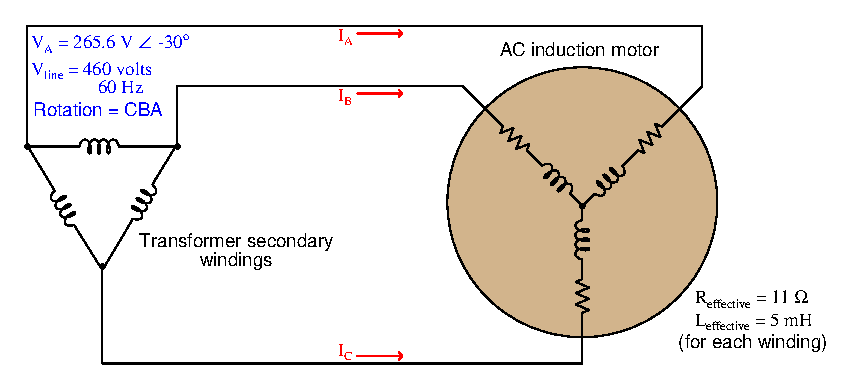
\includegraphics[width=15.5cm]{i00830x01.eps}$$

\underbar{file i00830}
%(END_QUESTION)





%(BEGIN_ANSWER)

$I_A = 23.79 \hbox{ A } \angle -39.72^o$

$I_B = 23.79 \hbox{ A } \angle -279.72^o$

$I_C = 23.79 \hbox{ A } \angle -159.72^o$


%(END_ANSWER)





%(BEGIN_NOTES)

Hvis $V_A$ (spenning i fase A mot jord) er 265.5 volt $\angle$ $-30^o$, og fasesekvensen er CBA (eller ACB), må fasespenningene være:

\begin{itemize}
\item{} $V_A$ = 265.5 volt $\angle$ $-30^o$
\item{} $V_C$ = 265.5 volt $\angle$ $-150^o$
\item{} $V_B$ = 265.5 volt $\angle$ $-270^o$
\end{itemize}

Beregning av hver linjestrøm gjøres ved å dele respektiv fasespenning på faseimpedansen:

$$Z_{phase} = 11 + j 2 \pi f L$$

$$Z_{phase} = 11 + j (2) (\pi) (60) (0.005)$$

$$Z_{phase} = 11 + j 1.885 \> \Omega = 11.16 \> \Omega \angle 9.72^o$$

\vskip 10pt

$$I_A = {{265.5 \hbox{ V } \angle -30^o} \over {11.16 \> \Omega \angle 9.72^o}} = 23.79 \hbox{ A } \angle -39.72^o$$

$$I_B = {{265.5 \hbox{ V } \angle -270^o} \over {11.16 \> \Omega \angle 9.72^o}} = 23.79 \hbox{ A } \angle -279.72^o$$

$$I_C = {{265.5 \hbox{ V } \angle -150^o} \over {11.16 \> \Omega \angle 9.72^o}} = 23.79 \hbox{ A } \angle -159.72^o$$

%INDEX% Electronics review: 3-phase voltage/current/power calculation
%INDEX% Electronics review: AC reactance and impedance
%INDEX% Electronics review, phasor expressions of circuit quantities
%INDEX% Electronics review: series and parallel AC circuits

%(END_NOTES)
